\pgfplotsset{yticklabel style={text width=5em,align=right}}
\begin{figure}[htb]

\resizebox{0.75\columnwidth}{!}{
\subfigure{
\begin{tikzpicture}[->,>=stealth',auto,node distance=3cm,
  thick,main node/.style={circle,draw,font=\sffamily\Large\bfseries}]
  \node[] at (-2,1) {\huge (a)};
\node[main node] (1) {};
\node[main node] (2) [right of=1] {};
\node[main node] (3) [right of=2] {};
\node[main node] (4) [right of=3] {};

\draw [->] (1) to [out=20, in=160] (2);
\draw [->] (2) to [out=20, in=160] (3);
\draw [->] (3) to [out=20, in=160] (4);
\draw [->] (2) -- (1);
\draw [->] (3) -- (2) ;
\draw [->] (4) -- (3);
\draw [->, red] (4) to [out=150,in=30] (1);
\draw [->,red] (1.north) to [out=30,in=150] (4.north);
\draw [->,red] (1) to [out=30,in=150, bend right=20] (3);
\draw [->,red] (3.south) to [out=150,in=30, bend left = 20] (1.south);
\draw [->,red] (2) to [out=30,in=150, bend right=20] (4);
\draw [->,red] (4.south) to [out=150,in=30, bend left = 20] (2.south);
\end{tikzpicture}}
}
\resizebox{0.76\columnwidth}{!}{
\subfigure{
\begin{tikzpicture}
\node[] at (-2,7) {\huge (b)};

\begin{axis}[%
%width=4in,
%height=4in,
%at={(0in,0in)},
scale only axis,
xmin=1,
xmax=10,
xtick={1,3,5,7,9},
xlabel style={font=\huge\color{white!15!black}},
xlabel={$r = k/l$},
ymin=0,
ymax=0.55,
ytick={0.1,0.3,0.5},
ylabel style={font=\huge\color{white!15!black}, at={(axis description cs:-0.15,0.5)}},
ylabel={$\Theta$},
axis background/.style={fill=white},
legend style={legend cell align=left, align=left, draw=white!15!black}
]
\addplot [color=black]
  table[row sep=crcr]{%
1	0.528595479208968\\
1.09090909090909	0.50147673688684\\
1.18181818181818	0.477019492251525\\
1.27272727272727	0.454895067403881\\
1.36363636363636	0.434816959975228\\
1.45454545454545	0.416537192638981\\
1.54545454545455	0.399841821547982\\
1.63636363636364	0.384546414763086\\
1.72727272727273	0.370491866810496\\
1.81818181818182	0.357540687167248\\
1.90909090909091	0.3455737869816\\
2	0.334487735353838\\
2.09090909090909	0.324192434963534\\
2.18181818181818	0.314609161188975\\
2.27272727272727	0.305668910853743\\
2.36363636363636	0.297311012007194\\
2.45454545454545	0.289481952467273\\
2.54545454545455	0.282134391129488\\
2.63636363636364	0.275226321781979\\
2.72727272727273	0.268720364185128\\
2.81818181818182	0.262583161453856\\
2.90909090909091	0.256784866374109\\
3	0.251298702273067\\
3.09090909090909	0.24610058653295\\
3.18181818181818	0.241168806873832\\
3.27272727272727	0.236483742205569\\
3.36363636363636	0.232027621226193\\
3.45454545454545	0.227784313077425\\
3.54545454545455	0.223739145301524\\
3.63636363636364	0.219878745113962\\
3.72727272727273	0.216190900643201\\
3.81818181818182	0.212664439316352\\
3.90909090909091	0.209289121007604\\
4	0.206055543930894\\
4.09090909090909	0.202955061562617\\
4.18181818181818	0.19997970913475\\
4.27272727272727	0.197122138452283\\
4.36363636363636	0.194375559968448\\
4.45454545454546	0.191733691202618\\
4.54545454545454	0.18919071071374\\
4.63636363636364	0.186741216950604\\
4.72727272727273	0.184380191392375\\
4.81818181818182	0.182102965471274\\
4.90909090909091	0.179905190836244\\
5	0.177782812573782\\
5.09090909090909	0.175732045051198\\
5.18181818181818	0.173749350089879\\
5.27272727272727	0.171831417212448\\
5.36363636363636	0.16997514573921\\
5.45454545454545	0.168177628536371\\
5.54545454545455	0.166436137242153\\
5.63636363636364	0.164748108817365\\
5.72727272727273	0.163111133284805\\
5.81818181818182	0.161522942537425\\
5.90909090909091	0.159981400108769\\
6	0.158484491811051\\
6.09090909090909	0.157030317156709\\
6.18181818181818	0.155617081488386\\
6.27272727272727	0.15424308875037\\
6.36363636363636	0.152906734841615\\
6.45454545454545	0.151606501496755\\
6.54545454545455	0.150340950647027\\
6.63636363636364	0.149108719217995\\
6.72727272727273	0.147908514325239\\
6.81818181818182	0.146739108833137\\
6.90909090909091	0.145599337245228\\
7	0.144488091897757\\
7.09090909090909	0.143404319430742\\
7.18181818181818	0.142347017513314\\
7.27272727272727	0.141315231802305\\
7.36363636363636	0.140308053114993\\
7.45454545454545	0.139324614798688\\
7.54545454545455	0.138364090281396\\
7.63636363636364	0.13742569078925\\
7.72727272727273	0.136508663217644\\
7.81818181818182	0.135612288144175\\
7.90909090909091	0.13473587797252\\
8	0.133878775197339\\
8.09090909090909	0.13304035078111\\
8.18181818181818	0.132220002634592\\
8.27272727272727	0.13141715419331\\
8.36363636363636	0.130631253083061\\
8.45454545454545	0.129861769868044\\
8.54545454545455	0.129108196875724\\
8.63636363636364	0.128370047093001\\
8.72727272727273	0.127646853128714\\
8.81818181818182	0.126938166237881\\
8.90909090909091	0.126243555403441\\
9	0.125562606471598\\
9.09090909090909	0.124894921337152\\
9.18181818181818	0.124240117175503\\
9.27272727272727	0.123597825718219\\
9.36363636363636	0.122967692569348\\
9.45454545454546	0.122349376559807\\
9.54545454545454	0.12174254913742\\
9.63636363636364	0.121146893790321\\
9.72727272727273	0.120562105501626\\
9.81818181818182	0.119987890233413\\
9.90909090909091	0.119423964438198\\
10	0.118870054596202\\
};
\end{axis}
\end{tikzpicture}}
}
%\resizebox{0.75\columnwidth}{!}{
%\subfigure{
%% This file was created by matlab2tikz.
%
%The latest updates can be retrieved from
%  http://www.mathworks.com/matlabcentral/fileexchange/22022-matlab2tikz-matlab2tikz
%where you can also make suggestions and rate matlab2tikz.
%
\definecolor{mycolor1}{rgb}{0.00000,0.44700,0.74100}%
%
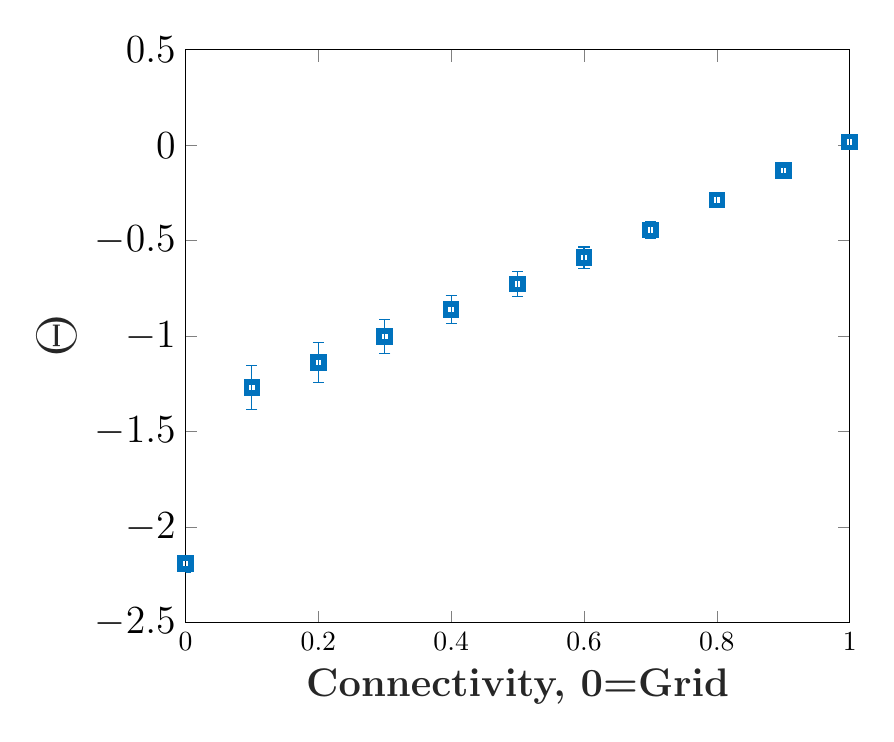
\begin{tikzpicture}
%\node[] at (-2,7) {\huge (b)};

\begin{axis}[%
%width=4in,
%height=4in,
%at={(0in,0in)},
scale only axis,
xmin=0,
xmax=1,
xtick={0, 0.2, 0.4, 0.6, 0.8, 1},
xlabel style={font=\Large\bfseries\color{white!15!black}},
xlabel={Connectivity, 0=Grid},
ymin=-2.5,
ymax=0.5,
yticklabel style = {font=\Large},
ylabel style={font=\huge\bfseries\color{white!15!black}, at={(axis description cs:-0.15,0.5)}},
scale ticks below exponent=2,
ylabel={$\Theta$},
axis background/.style={fill=white},
legend style={legend cell align=left, align=left, draw=white!15!black}
]
\addplot [color=mycolor1, line width=2.0pt, draw=none, mark=square, mark options={solid, mycolor1}]
 plot [error bars/.cd, y dir = both, y explicit]
 table[row sep=crcr, y error plus index=2, y error minus index=3]{%
1	0.0158897932895343	0.0219638609519872	0.0219638609519872\\
0	-2.19152922410445	0.0442727133533317	0.0442727133533317\\
0.1	-1.26900238075602	0.113140127221996	0.113140127221996\\
0.2	-1.13717407560137	0.105399483670646	0.105399483670646\\
0.3	-1.00117652331271	0.088778703694582	0.088778703694582\\
0.4	-0.860142584690047	0.0752706537627627	0.0752706537627627\\
0.5	-0.726084325807173	0.0648688752958107	0.0648688752958107\\
0.6	-0.588945001891375	0.0557394993663173	0.0557394993663173\\
0.7	-0.444804928347819	0.0432954017554721	0.0432954017554721\\
0.8	-0.287006316742788	0.0332660232213172	0.0332660232213172\\
0.9	-0.132989953746229	0.0271438744901984	0.0271438744901984\\
};

\end{axis}

\end{tikzpicture}%
}
%}
\caption{Orthogonality captures the number of effective pathways directed at discriminatory nodes.  (a) A toy four-node discriminatory scheme.  (b) When each black and red arrow in panel (a) has weight $k, \ l$ (respectively) we find that the orthogonality ($\Theta$) decreases as the black arrows dominate, creating a singly dominant path.  Note that the $x$-axis begins at $r=1,$ corresponding to an all-to-all connected graph with equal weights.\label{fig:toy_model}}
\end{figure}


%As connections of equal order of magnitude are deleted from an all-to-all connected graph, orthogonality decreases.  For each graph, a fraction of nodes were randomly deleted; error bars represent standard deviation of orthogonality over 1000 trials at each sparsity. At 0 is $\Theta(Grid)$ 